\begin{question}
\noindent Triangle $T$ is drawn on the grid below.

\begin{center}
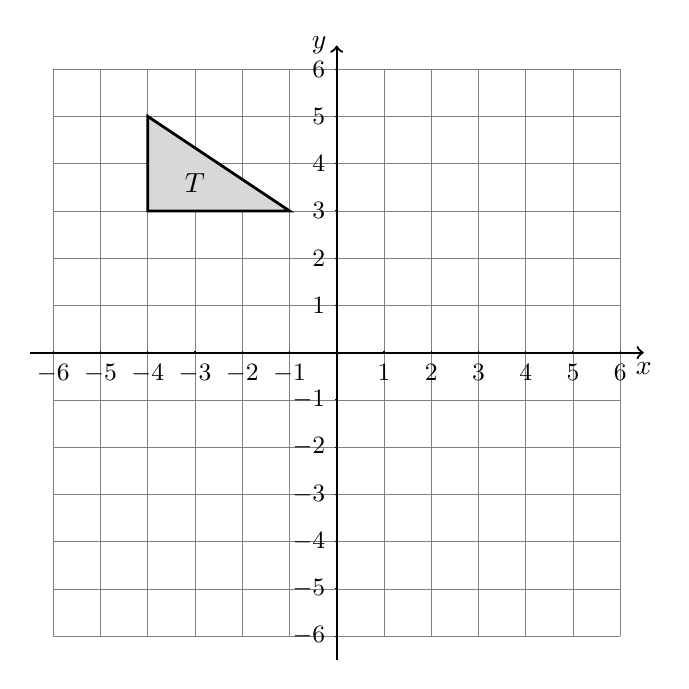
\begin{tikzpicture}[scale=0.6]
    % Define colours
    \definecolor{borderColour}{HTML}{000000}
    \definecolor{fillColour}{HTML}{D8D8D8}

    % Define axis scale
    \def\axisLimit{6}

    % Draw the grid
    \draw[step=1cm,gray,very thin] (-\axisLimit,-\axisLimit) grid (\axisLimit,\axisLimit);
    \draw[thick,->] (-\axisLimit-0.5,0) -- (\axisLimit+0.5,0) node[anchor=north] {$x$};
    \draw[thick,->] (0,-\axisLimit-0.5) -- (0,\axisLimit+0.5) node[anchor=east] {$y$};

    % Label x-axis and y-axis
    \foreach \x in {-6,-5,...,-1,1,2,...,6}
        \draw (\x cm,1pt) -- (\x cm,-1pt) node[anchor=north] {\small $\x$};
    \foreach \y in {-6,-5,...,-1,1,2,...,6}
        \draw (1pt,\y cm) -- (-1pt,\y cm) node[anchor=east] {\small $\y$};

    % Define the vertices of triangle T
    \coordinate (A) at (-4,3);
    \coordinate (B) at (-4,5);
    \coordinate (C) at (-1,3);

    % Draw triangle T
    \filldraw[fill=fillColour, draw=borderColour, line width=1pt] (A) -- (B) -- (C) -- cycle;

    % Label the triangle and vertices
    \node at (-3,3.6) {$T$};

\end{tikzpicture}
\end{center}

\noindent Triangle $T$ is translated by the vector $\begin{pmatrix} 3 \\ -2 \end{pmatrix}$ to give triangle $T'$.

\noindent Find the coordinates of the vertices of triangle $T'$.

\vspace{4cm}
\begin{flushright}
\answerplain{2}
\end{flushright}
\end{question}
